\documentclass[12pt]{article}
\usepackage{amsmath}
\usepackage{fancyhdr}
\usepackage{hyperref}
\usepackage{graphicx}
\newcommand{\compactlist}{\setlength{\itemsep}{0pt} \setlength{\parskip}{0pt} \setlength{\leftskip}{-1em}}
\usepackage[top=0.9in, bottom=0.8in, left=0.9in, right=0.9in]{geometry}

\lhead{MATH 4263/5373}
\rhead{Sep. 5, 2019}
\chead[RE]{Fixed-point iterations: II}
\cfoot{}
%\rfoot{Code for figure and report is (not yet) available in the class folder.}
\pagestyle{fancy}

\begin{document}
Consider the fixed-point problems \(\sin(x) = x\) (below, left) and \(\cos(x) = x\) (below, right).
%
\begin{center}
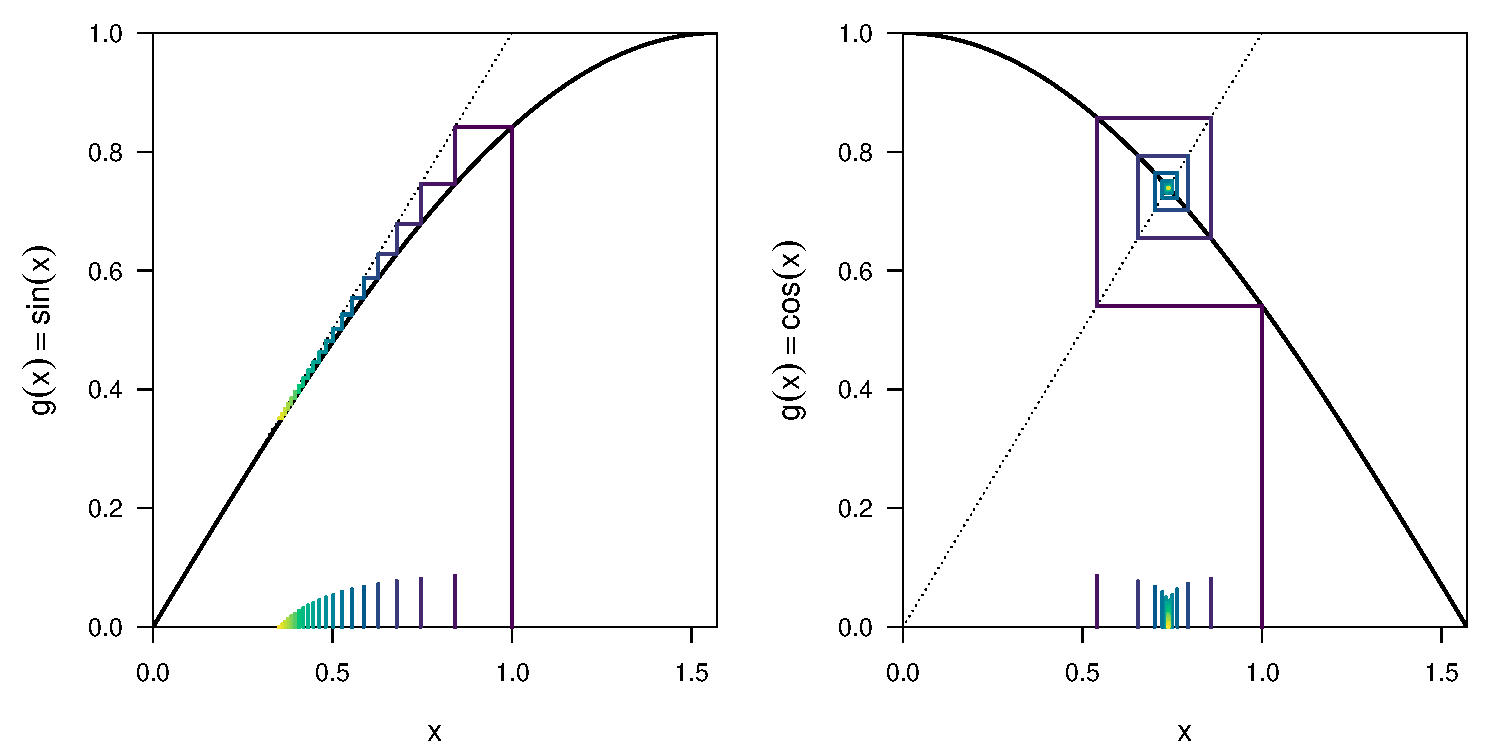
\includegraphics[width=0.95\textwidth]{fixpt_trig.pdf}
\end{center}
%
A total of \(20\) iterations of each problem are shown in the color figure above.  Time is indicated in two ways: on the graph early steps are in dark blue and fade to yellow.  Along the axis earlier approximations are marked by tall (also dark blue) tick marks and later iterations are marked by shorter (also yellow) tick marks.  The scaling of the above-axis tick marks is nothing quantitative or necessarily related to the values of the approximation itself, it is just meant to show the progression of the iterations.

For two problems starting from \(p_0=1\), we see the iterations approaching the fixed point visible on each panel of the graph.  Solutions to the first fixed-point problem (left) converge very slowly, while those to the second (right) converge very quickly.  Details of the approaches to the fixed points are interesting as well.  Approximations converging to the true solution of \(p=0\) for the first problem decrease monotonically, while those converging to the true solution of the second problem oscillate.

\paragraph{Challenge} For each of the above, state an associated rootfinding problem, an interval on which you could apply the bisection method, and the number of iterations it would take to approximate the root to an accuracy of \(10^{-6}\) with bisection.
\end{document}

%:
%:
%:
%:
%:
%:
